Since the appearance of the first digital computers in 1940s, Monte Carlo (MC) sampling remains one of the most well-known and widely used methods of the analysis of stochastic systems.
The reason for this popularity lies in the ease of implementation, in the independence of the stochastic dimensionality of the considered problems, and in the fact that the quantities estimated using MC simulations are guaranteed to converge to the true values by the central limit theorem \cite{durrett2010}.
The major problem with MC sampling, however, is the low rate of convergence, \eg, the mean value converges as $\nsamples^{-\ifrac{1}{2}}$ where $\nsamples$ is the number of samples \cite{xiu2010, maitre2010}.
This means that, in order to get an additional decimal point of accuracy, one has to obtain hundred times more samples.
Each such sample implies a complete realization of the whole system, which makes MC-based methods slow and often infeasible since the number of needed simulations can be extremely large \cite{diaz-emparanza2002}.

In order to overcome the limitations of deterministic power-temperature analysis (PTA) and, at the same time, to completely eliminate or, at least, to mitigate the costs associated with MC sampling, a number of alternative stochastic PTA techniques have been recently introduced.
Since the leakage power is influenced by process variation the most \cite{chandrakasan2001, srivastava2010, juan2011, juan2012}, the techniques discussed below primarily focus on the variability of leakage, which we shall also do.

A solely power-targeted but temperature-aware solution is proposed in \cite{chandra2010} wherein the driving force of the analysis is MC simulations with partially precomputed data.
A learning-based approach is presented in \cite{juan2011} to estimate the maximal temperature under the steady-state condition.
Temperature-related issues originating from process variation are also considered in \cite{juan2012} where a statistical model of the steady-state temperature based on Gaussian distributions is derived.
In \cite{shen2009}, the theory of polynomial chaos (PC) expansions \cite{xiu2010, maitre2010, ghanem1991, eldred2009} together with principal component analysis (PCA) are employed to estimate the full-chip leakage power.
A generalization of PCA known as the Karhunen-Lo\`{e}ve (KL) decomposition (refer to the same literature as for PC mentioned above) is used in \cite{bhardwaj2006} for the leakage calculation.
An analysis of the voltage response of power grids is carried out in \cite{ghanta2006} where the PC and KL methods are jointly utilized. The last three techniques, \ie, \cite{shen2009, bhardwaj2006, ghanta2006}, are temperature-unaware solutions to power modeling under process variation.

\begin{figure}[br]
  \vspace{-1.5em}
  \centering
  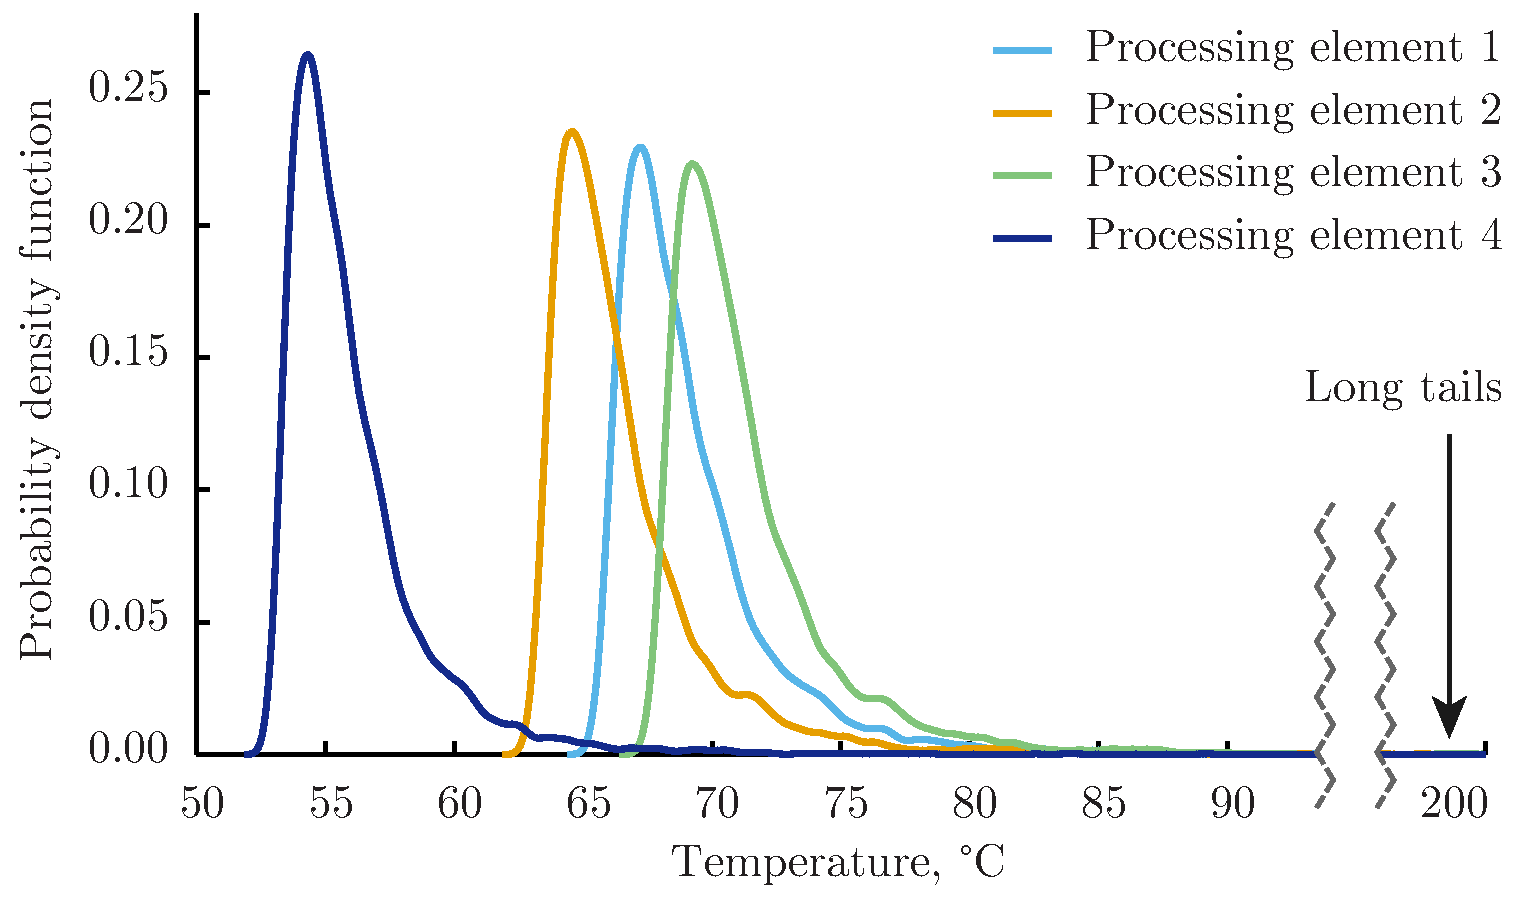
\includegraphics[width=1.0\linewidth]{include/assets/motivation-pdf.pdf}
  \caption{Probability density functions.}
  \flabel{motivation-pdf}
  \vspace{-1.0em}
\end{figure}

None of the aforementioned power- and/or temperature-related techniques attempts to perform stochastic transient PTA and to compute the evolving-in-time probability distribution of temperature.
However, such transient curves are of practical importance.
First of all, certain procedures cannot be undertaken without the knowledge of time-dependent temperature variations, \eg, the reliability optimization based on the thermal-cycling fatigue. Secondly, the constant steady-state temperature assumption, considered, \eg, in \cite{juan2011, juan2012}, can rarely be justified since power profiles are not invariant in reality.
Moreover, the frequently made assumption that power and/or temperature follow \apriori\ known probability distributions---for instance, Gaussian and log-normal distributions are popular choices, as in \cite{srivastava2010, juan2012, bhardwaj2006}---is not realistic due to (a) the strict nonlinearities between the process parameters, power, and temperature; (b) the nonlinear interdependency of temperature and the leakage power \cite{liu2007}.
To illustrate this, we simulated the previously mentioned example $10^4$ times as it is further discussed in \sref{illustrative-example}, and performed kernel density estimation of probability density functions (\pdfs) of the temperature of the four processors at the middle of the time span shown in \fref{motivation-curve} (at time 0.39~s).
The results are depicted in \fref{motivation-pdf}. It can be seen that they are neither Gaussian, as the obtained curves do not even closely resemble the well-known bell-shaped curves of Gaussian distributions, nor log-normal, as the curves in \fref{motivation-pdf} have thin tails, which is opposed to the heavy tails of log-normal distributions.

To conclude, the present stochastic PTA techniques for multiprocessor system design are restricted in use due to one or several of the following traits: based on MC simulations (potentially slow) \cite{chandra2010}, limited to power analysis \cite{chandra2010, shen2009, bhardwaj2006, ghanta2006}, limited to the assumption of the constant steady-state temperature \cite{juan2011, juan2012}, exclusive focus on the maximal temperature \cite{juan2011}, \apriori\ chosen distributions of power and temperature \cite{srivastava2010, juan2012, bhardwaj2006}.
Consequently, there is a lack of flexible stochastic PTA techniques, which we aim to fulfill.
